\documentclass[letter paper, title page]{article}
\usepackage{graphicx} % Required for inserting images
\usepackage[capposition=top]{floatrow}
\usepackage[margin=1in]{geometry}
\usepackage[export]{adjustbox}
\usepackage{tabularx}
\usepackage{multirow}
\usepackage{amssymb}

\title{\huge Physics 55 - Lab 6: Force Table}
\author{Andrew Card, Preston Kearnan, Roan Morgan, Michael Roberts}
\date{February 2, 2023}

\begin{document}

\maketitle

\noindent
\title{\huge Equilibrium} \\

\noindent
\title{Objective}

\begin{list}
    \\\item - The Objective of today's lab is to utilize Newton's 2nd law and solve force related problems to further our understanding of "Static Equilibrium". 
\end{list}

\section*{Three Forces}

\noindent
\title{\textbf{Synopsis}}

\begin{list}
    \\\item - We will first record the angle and force required to balance our table.

            - We will Create a table and free body diagram of our findings

            - We will add our forces to test our "Equilibrium"

            - We will use math to find and add the remaining forces into one vector \\
\end{list}

\noindent
\title{\textbf{Angle and Spring Tension Table}} \\

\noindent

\begin{tabular}{|c c c c|}

\hline
  & String 1 & String 2 & String 3\\
 \hline\hline
 Tension & 150g ± 5g & 150g ± 5g & 185g ± 5g \\
 \hline
 Angle & 0\textdegree & 90\textdegree & 240\textdegree ± 3\textdegree \\
 \hline

\end{tabular} \\

\begin{figure}[H]
    \centering
    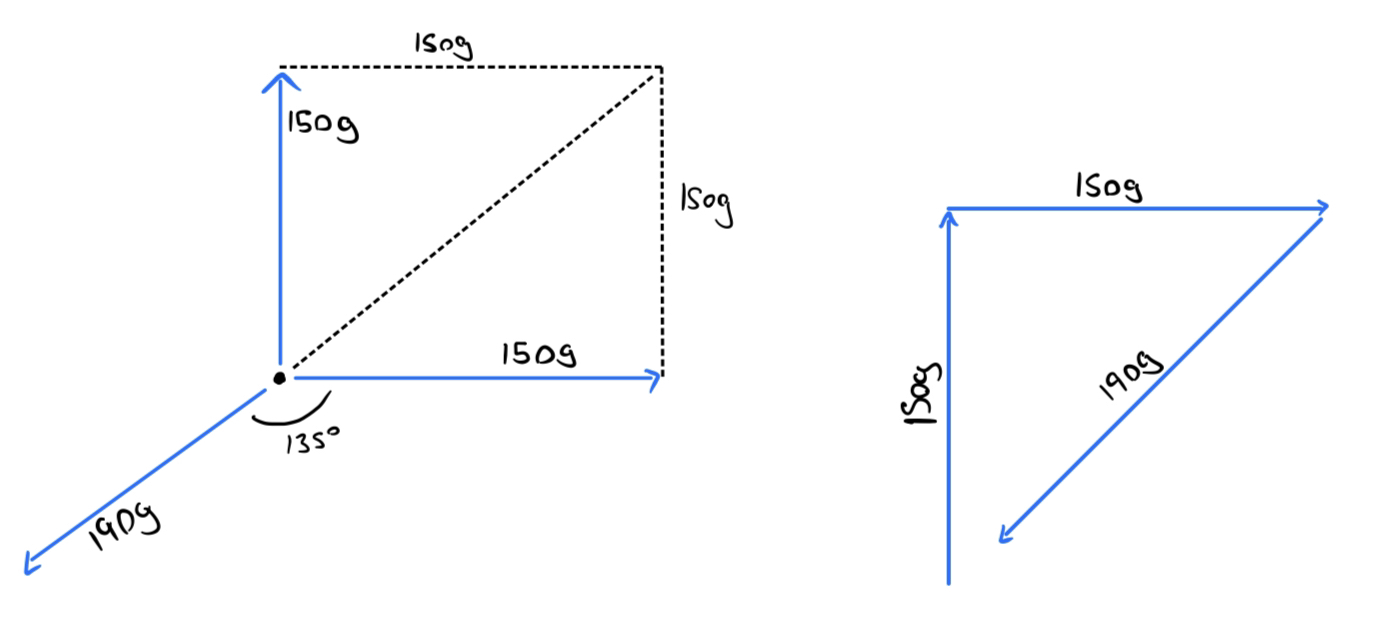
\includegraphics[scale = 0.2]{freebody-tiptotail.jpg}
    \caption{FBD \& Tip - Tail}
    \label{fig:my_label}
\end{figure}

\noindent
\title{\textbf{Force Summation}}

\begin{list}
    \list \\ - After our calculations and experiments, the combined net force in the x direction that we solved for was just 2.13N away from 0, and 0.50N away from 0 in the y direction. (Tip to Tail method seen above). 
\end{list}

\noindent
\title{\textbf{Observations}}

\begin{list}
    \\\item - The discrepancy in the net force can be accounted for in a few ways. However, it is Mostly likely caused by a slight error in the placement of the string, the reading of the scale, or the scale itself. 
\end{list}

\newpage

\section*{Four Forces, One Unknown Force}

\noindent
\title{\textbf{Synopsis}}

\begin{list}
    \\\item - We will draw a free-body diagram for our 3 known forces and find their components

            - We will find the magnitude and angle of the fourth force required.

            - We will then put our mathematical findings to the test experimentally. \\ 
\end{list}

\begin{figure}[H]
    \centering
    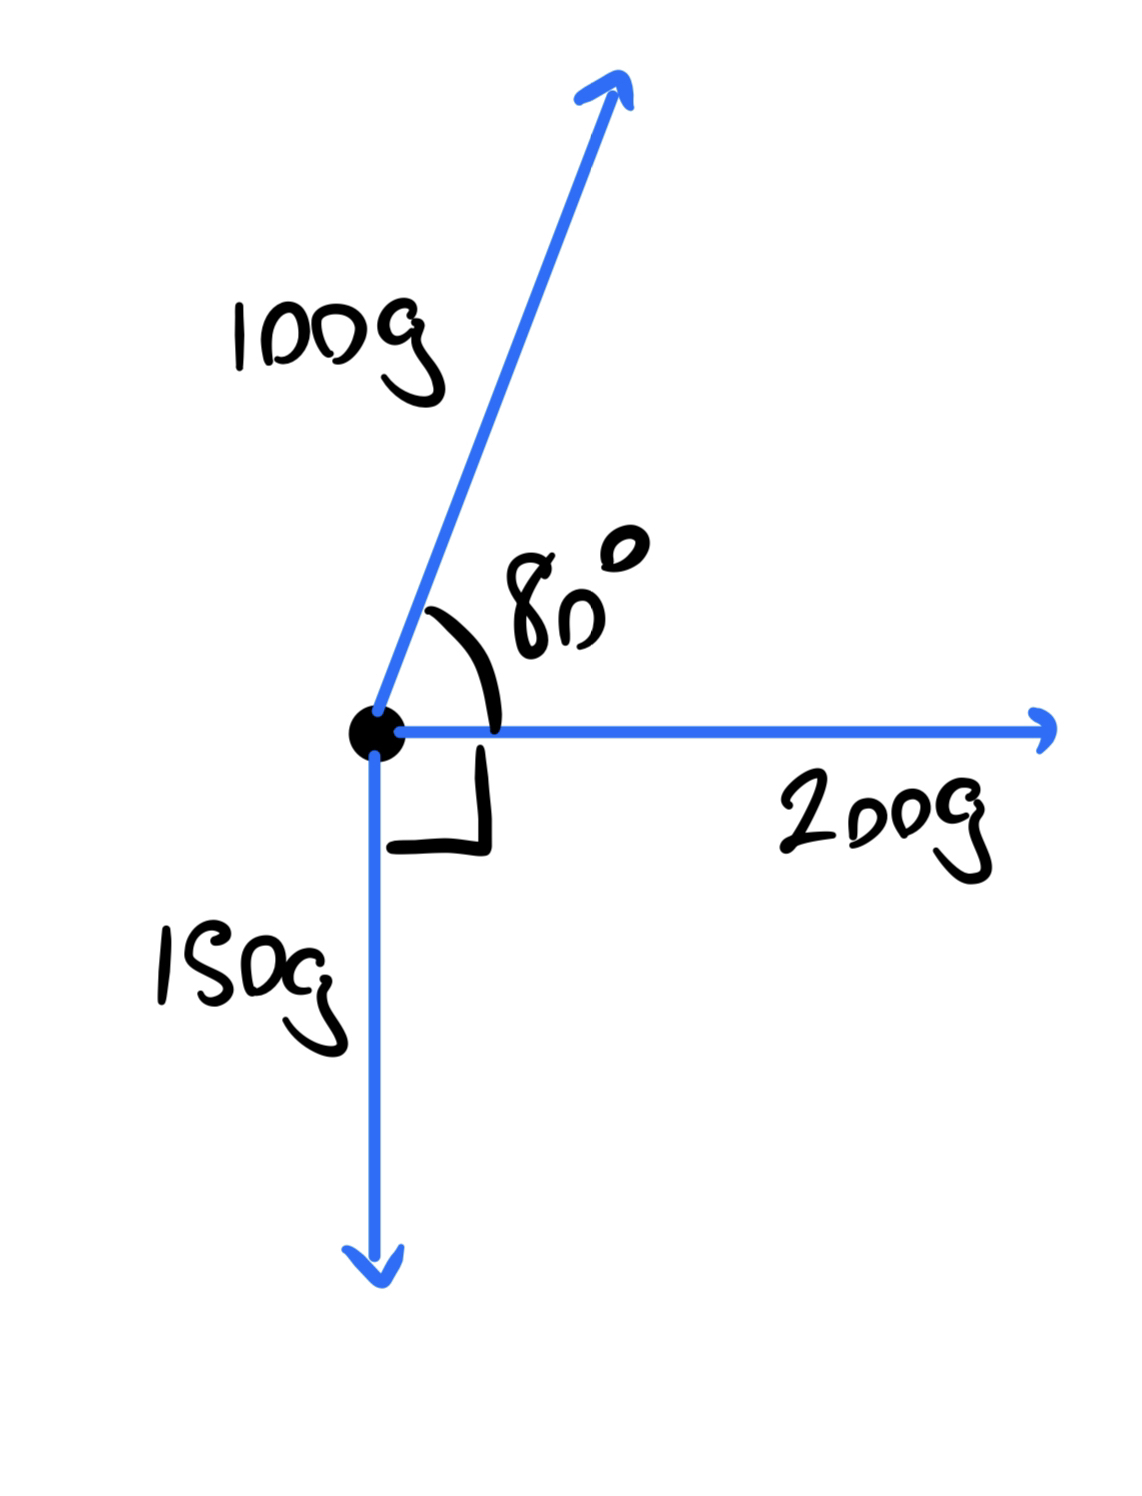
\includegraphics[scale = 0.1]{FBDQ6.jpg}
    \caption{FBD}
    \label{fig:my_label}
\end{figure}

\begin{list}
    \\ \item - The net x component caused by the forces is 2.13 Newtons. the net y component caused by the forces is -0.50 Newtons.  \\
\end{list}

\noindent
\title{\textbf{Fourth Force Calculations \\}}

\begin{tabular}{|c | c|}

\hline
  Mass (g) & Magnitude\\
 \hline
  223.645g & 2.19N\\
 \hline

\end{tabular} \\

\noindent
\title{\textbf{System Balance \\}}

\begin{tabular}{|c | c | c |}

\hline
 & Tension (N) & Angle\\
 \hline
 Calculated & N & 166.79\textdegree \\
 \hline
 Experimental & 2.19N & 166.6\textdegree \\
 \hline

\end{tabular}

\begin{list}
    \\ \list - Percent Error = 0.12\%
\end{list}

\noindent
\title{\textbf{Observations}}

\begin{list}
    \\\item - The difference between our calculations and reality are very similar, and the error is so low its almost negligible. 
\end{list}

\newpage

\section*{Four Forces, Two Unknown Angles}

\noindent
\title{\textbf{Synopsis}}

\begin{list}
    \\\item - We will determine the two unknown angles for balancing

            - We will draw a free body diagram and calculate the net forces on the ring \\
\end{list}

\noindent
\title{\textbf{Angles of Unknowns}} \\

\begin{tabular}{|c c c c c|}

\hline
  & String 1 & String 2 & String 3 & String 4 \\
 \hline\hline
 Tension & 250g & 150g & 150g ± 5g & 100g ± 5g \\
 \hline
 Angle & 0\textdegree & 150\textdegree & 170\textdegree ± 3\textdegree & 285\textdegree ± 3\textdegree \\
 \hline

\end{tabular} \\

\begin{figure}[H]
    \centering
    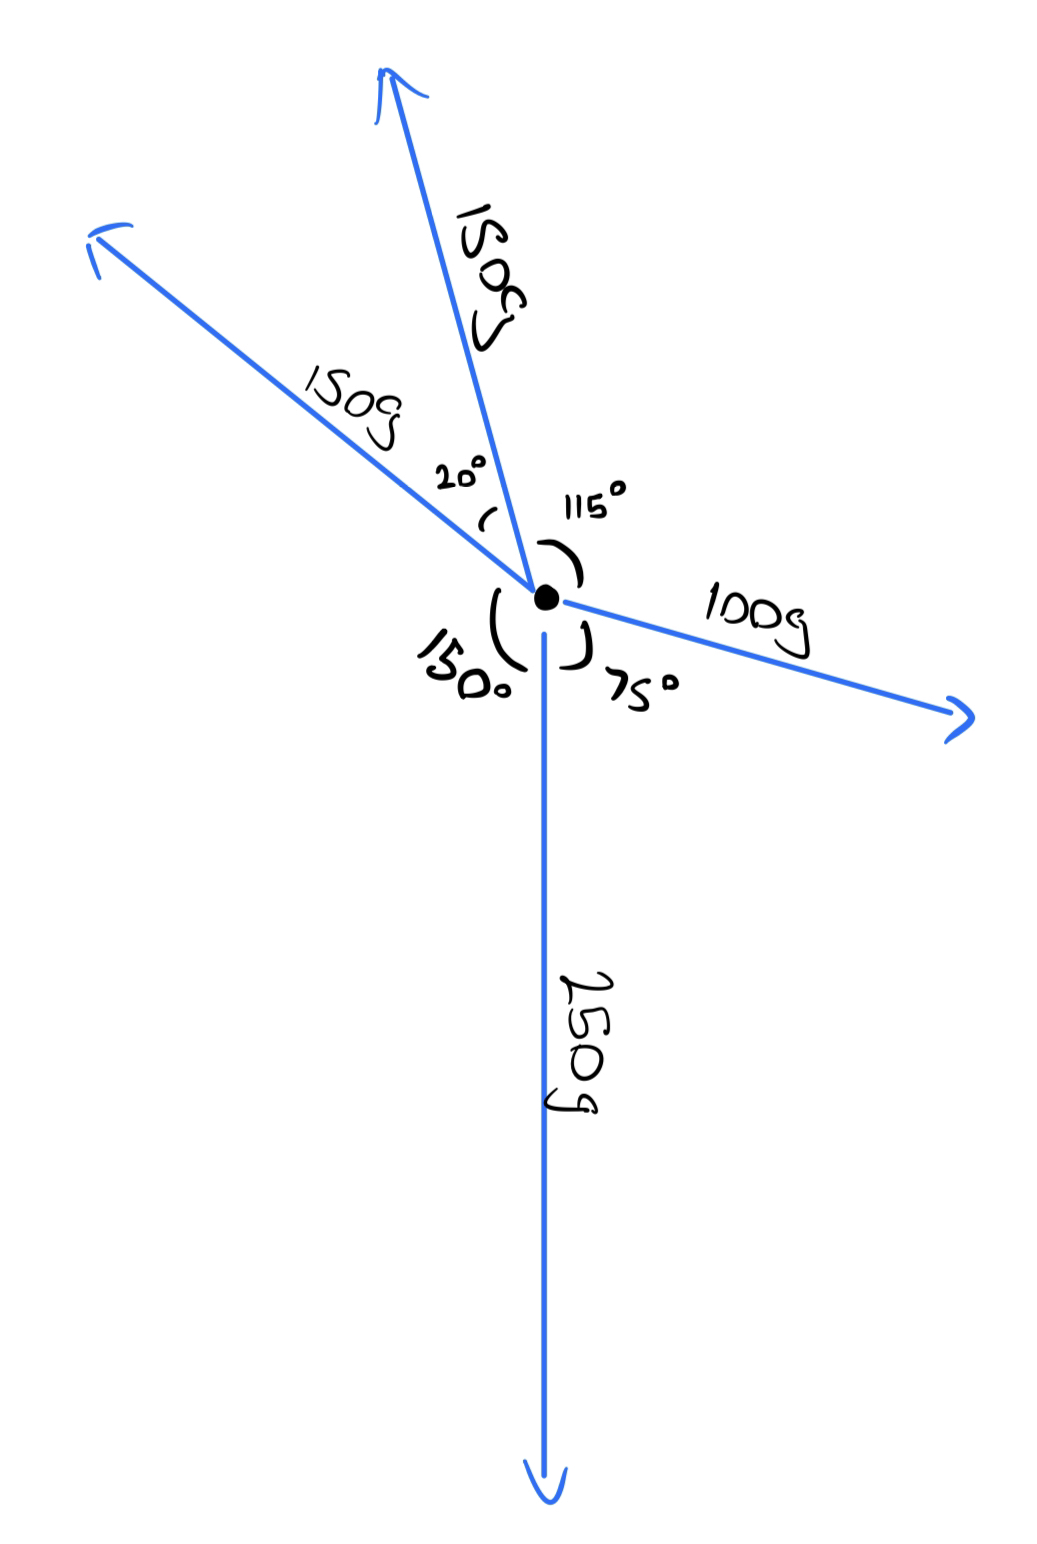
\includegraphics[scale = 0.1]{fbd9.jpg}
    \caption{FBD}
    \label{fig:my_label}
\end{figure}

\noindent
\title{\textbf{Alternate Methods}}

\begin{list}
    \\\item - There are a few ways to solve this problem. Obviously, the way that we solve this problem experimentally is one way to approach it. Using a force table and spring scale to physically find the answer. Another  way you could solve this problem is by using mathematics. Using kinematics and force summations to find the correct angle needed to balance the forces. Theoretically, the answer should be the same no matter which way you solve it, despite possible slight errors obtained in the experimental path. Given the fact that we have the ability to move two of the angles, there could be a multitude of angle combinations that give us the correct net force, 0. 
\end{list}

\noindent
\title{\textbf{Observations}}

\begin{list}
    \\\item - Content
\end{list}

\newpage

\section*{Extending the Range of the Spring Scale}

\noindent
\title{\textbf{Synopsis}}

\begin{list}
    \\\item - We will sketch a free body diagram of the rock-pulley system

            - Using our values measures we will determine the mass of the rock. 
\end{list}

\noindent
\title{\textbf{Equations/Diagrams}}

\begin{figure}[H]
    \centering
    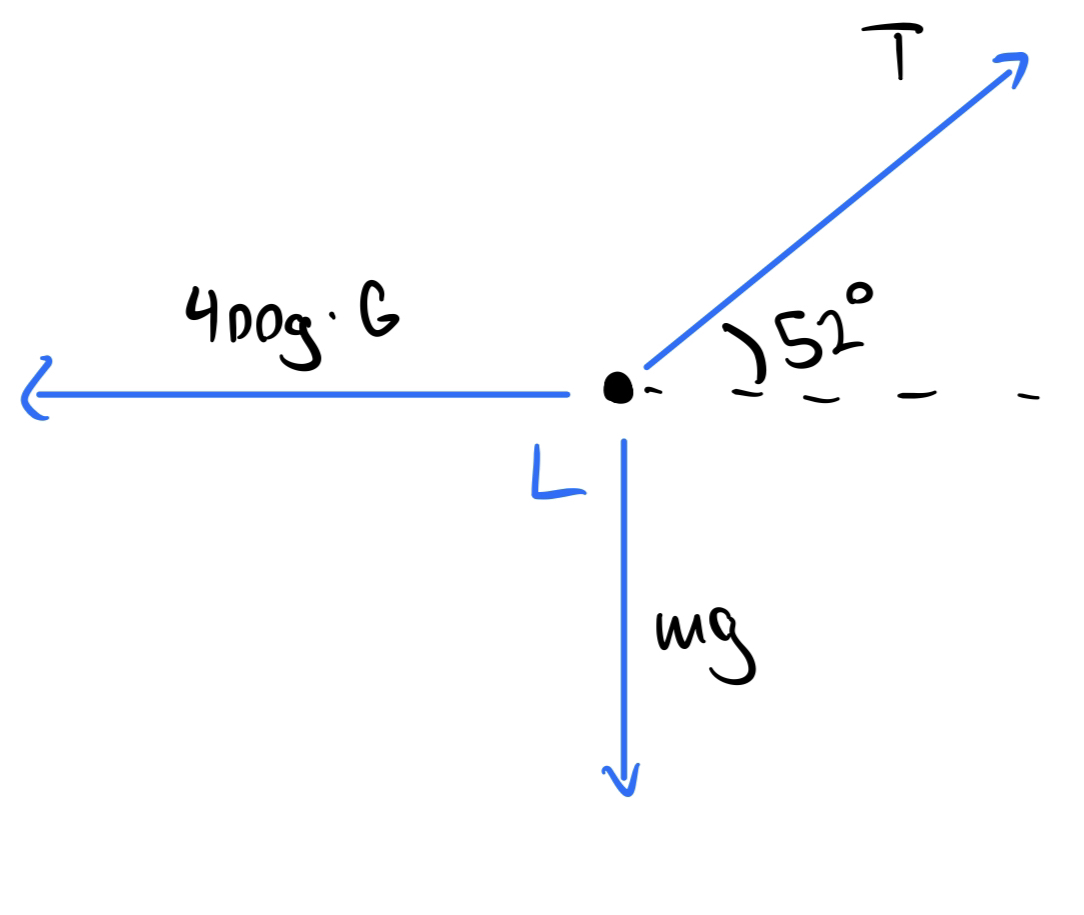
\includegraphics[scale = 0.1]{IMG_0057.png}
    \caption{FBD}
    \label{fig:my_label}
\end{figure}

\begin{figure}[H]
    \centering
    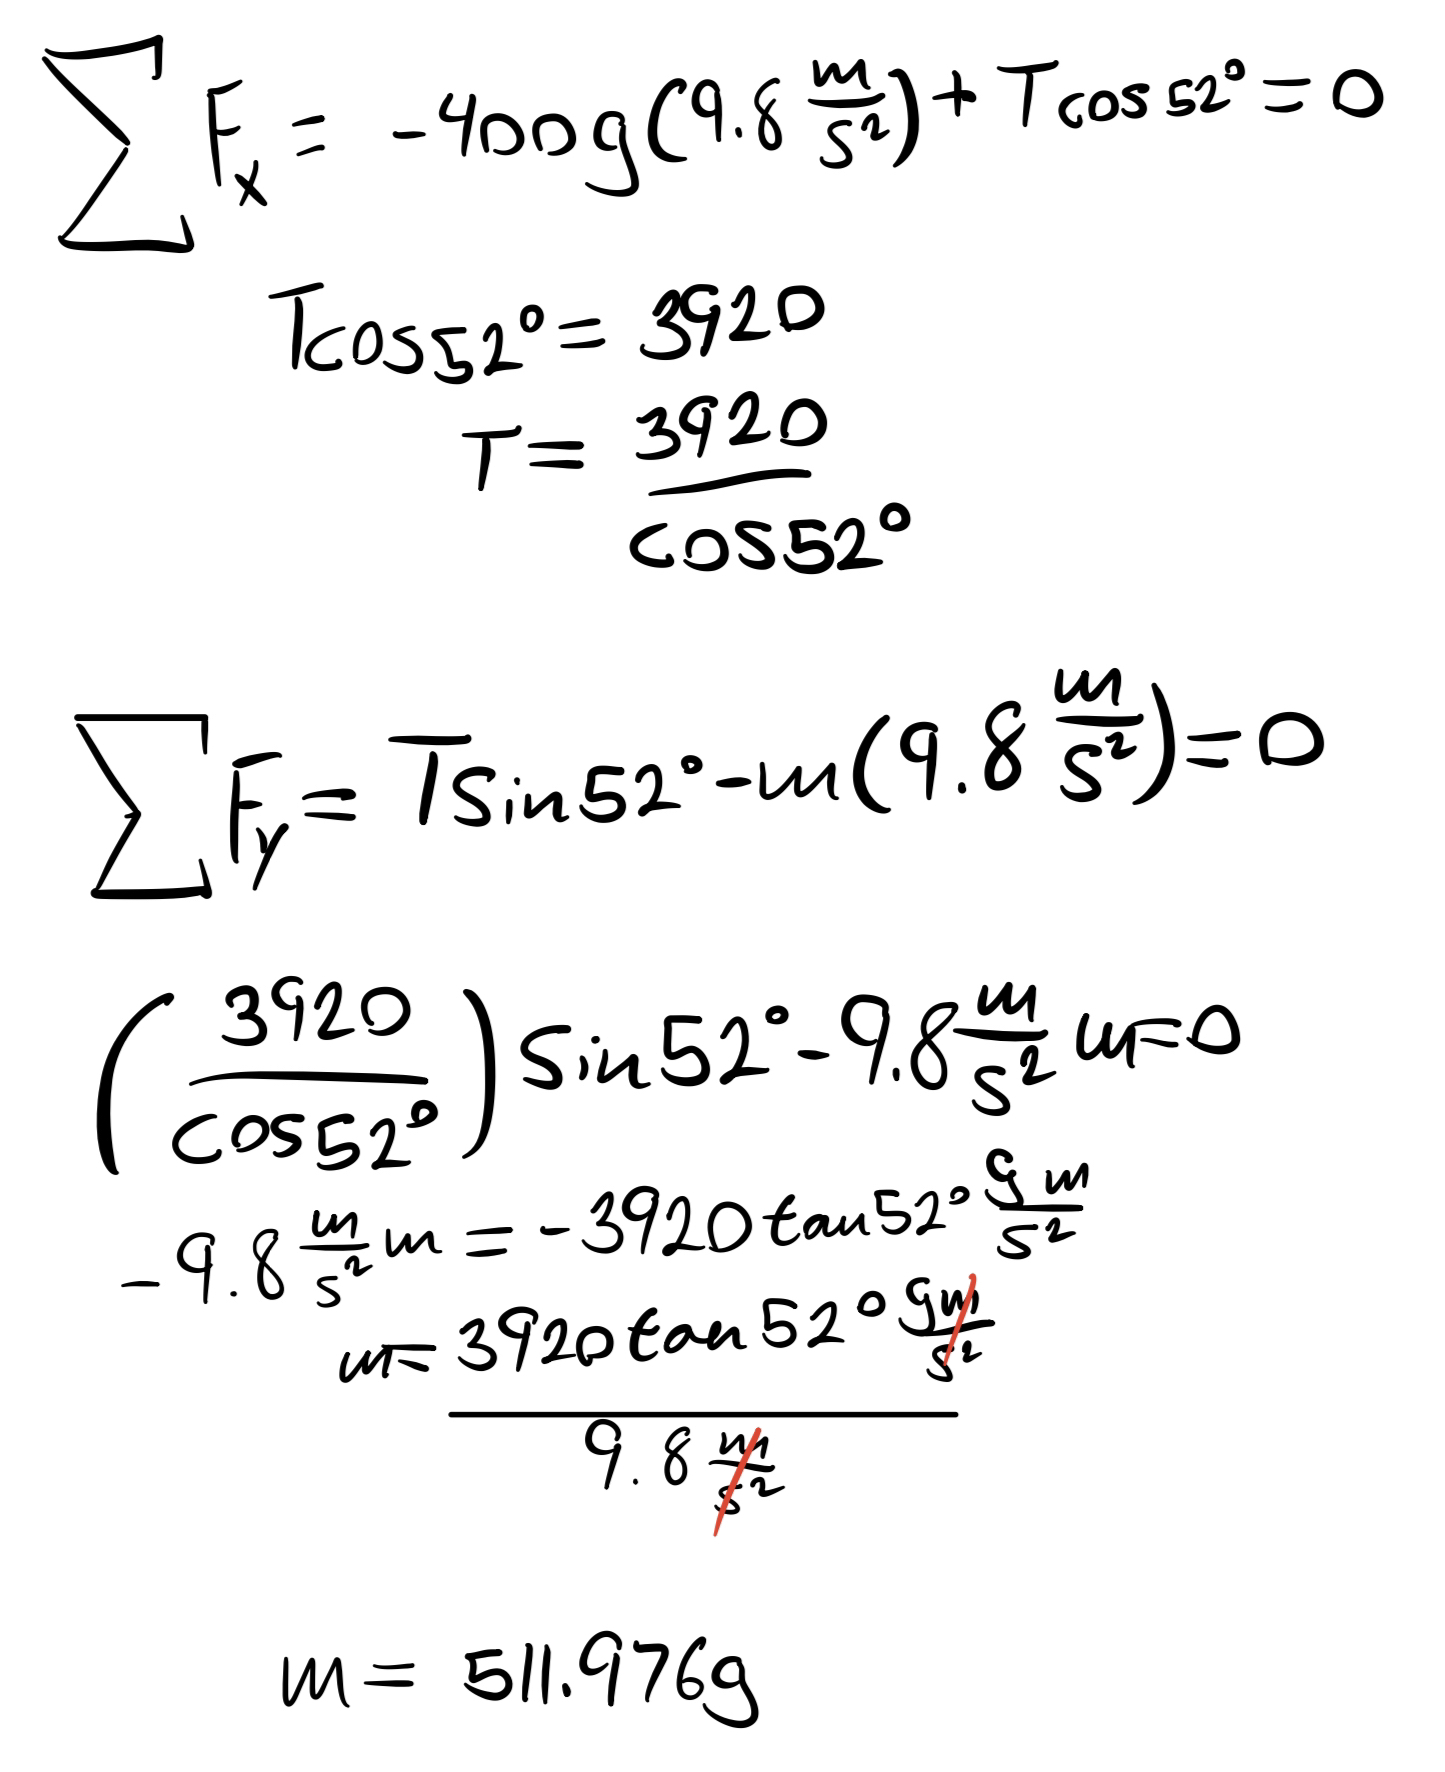
\includegraphics[scale = 0.15]{4EQTNS.jpg}
    \caption{Equations}
    \label{fig:my_label}
\end{figure}

\noindent
\title{Observations}

\begin{list}
    \\\item - Through this experiment, we learned that using angles, it is possible to measure the mass of an object using a scale that the object's mass exceeds. Overall we observed that small measuring mistakes can lead to crucial errors in final answers as we were not able to get the exact rock weight. 
\end{list}

\newpage

\section*{\textbf{Abstract}}

\begin{list}
    \\\item - In this lab, we discovered how we could use our newfound knowledge of forces in order to further understand the world around us. Deepening our understanding of forces and how they interact with each other has allowed us to come up with unique and innovative solutions to complex force-related problems. Using our knowledge of how forces interact and are altered by the angle at which they are enforced, we more confidently approach the world of physics and tackle all things "force" that come our way.  
\end{list}

\end{document}


